\documentclass[12pt]{article}
\usepackage{hyperref}
\usepackage[a4paper]{geometry}
\usepackage{graphicx}
\usepackage{listings}
\usepackage{multirow}

\newcommand{\fitxategi}[1] {\underline{\textit{#1}}}
\newcommand{\tekla}[1] {\textbf{#1}}

\renewcommand{\contentsname}{Edukiak}
\renewcommand{\refname}{Erreferentziak}


\geometry{
 a4paper,
 total={170mm,257mm},
 left=2cm,
 top=2cm,
 }


\title{KbG proiektua: 2. fasea}
\author{
        Oier Irazabal\\
        Jesus Calleja
}
\date{\today}



\begin{document}
\maketitle

%\begin{abstract}
%This is the paper's abstract \ldots
%\end{abstract}

\tableofcontents

\vspace{2cm}
\begin{center}
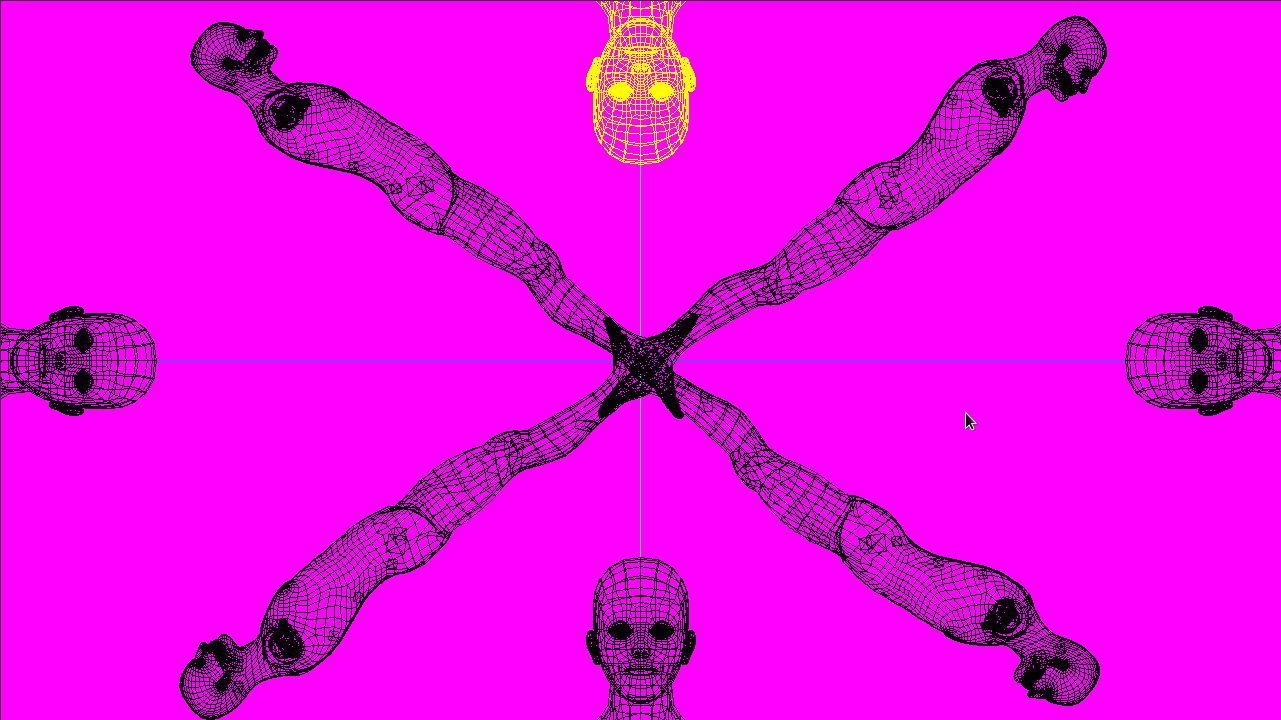
\includegraphics[scale=0.35]{kaizo.png}\\
\end{center}

\pagebreak



\section{Inplementazio berriak}

\subsection{Objektuen transformazioak}\label{transformazioak}

Hiru oinarrizko transformazioak (translazioa, errotazioa eta eskalaketa) inplementatu ditugu, erreferentzia-sistema globala zein lokala izanik.
Bai transformazio mota, bai erreferentzia-sistema automata baten bidez kodetuta daude. Automataren egoera batetik beste batera mugitzeko taula hauetan jasotako teklak sakatu behar dira:\\

\begin{center}

\begin{tabular}{|c|c|}
																				\hline
	Tekla							& Ekintza									\\	\hline
	\textbf{M} edo \textbf{m}		& Translazioa aktibatu						\\	\hline
	\textbf{B} edo \textbf{b}		& Biraketa aktibatu							\\	\hline
	\textbf{T} edo \textbf{t}		& Tamaina aldaketa aktibatu					\\	\hline
	\textbf{L} edo \textbf{l}		& Erreferentzia-sistema lokala aktibatu	\\	\hline
	\textbf{G} edo \textbf{g}		& Erreferentzia-sistema globala aktibatu	\\	\hline
	\textbf{+}						& Ardatz guztietan handitu objektua		\\	\hline
	\textbf{-}						& Ardatz guztietan handitu objektua		\\	\hline
\end{tabular}

\vspace{0.3cm}
1. Taula: Tekla arrunten taula
\end{center}

\begin{center}

\begin{tabular}{|c|c|c|c|}
																			\hline
	\multirow{3}{*}{Tekla}		& \multicolumn{3}{|c|}{Ekintza} 		\\	\cline{2-4}
	& Translazioaren  & Biraketaren  & Eskalaketaren 					\\ 
	&  norabidea &  ardatza &  norabidea 								\\	\hline
	\tekla{Goranzko gezia}		 &  Mugitu +Y & Biratu +X & Txikitu Y	\\	\hline
	\tekla{Beheranzko gezia}	 &  Mugitu -Y & Biratu -X & Handitu Y	\\	\hline
	\tekla{Ezkerreranzko gezia}&  Mugitu +X & Biratu +Y & Txikitu X	\\	\hline
	\tekla{Eskuineranzko gezia}&  Mugitu -X & Biratu -Y & Handitu X	\\	\hline
	\tekla{REPAG}				 &  Mugitu +Z & Biratu +Z & Txikitu Z	\\	\hline
	\tekla{AVPAG}				 &  Mugitu -Z & Biratu -Z & Handitu Z	\\	\hline
\end{tabular}

\vspace{0.3cm}
2. Taula: Tekla berezien taula
\end{center}


Beraz, automata honela geratuko litzaiguke:

\begin{center}
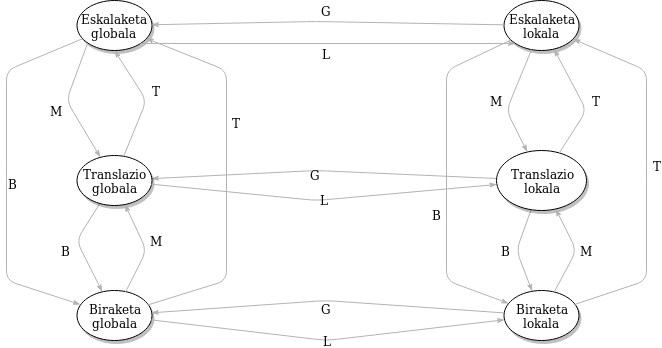
\includegraphics[scale=0.6]{egoeradiagrama.png}\\
\vspace{0.3cm}
1. Irudia: Egoera-diagrama
\end{center}


Transformazio-mota eta erreferentzia-sistema aldagai globalak \fitxategi{main.c}-n daude definituta eta hasieratuta translazio lokala burutzeko. Gainontzeko fitxategiek extern moduan erabili behar dituzte. Aldagai hauek hartu ditzaketen balioak \fitxategi{definizioak.h}-n daude definituta horrela:

\begin{center}
	\begin{lstlisting}[language=C, basicstyle=\footnotesize]
	#define TRANSLAZIOA                          0
	#define BIRAKETA                             1
	#define ESKALAKETA                           2
	
	#define LOKALA                               0
	#define GLOBALA                              1
	\end{lstlisting}
\end{center}


Orain, dena teorikoki definituta badaukagula, tekla bakoitza sakatzerakoan exekutatu behar den kodea bete behar da \fitxategi{io.c} fitxategian. 1. taulan jasotako teklek bakarrik esleitzen diote dagokion aldagaiari dagokion balioa, adibidez \tekla{m} teklaren kasuan:

\begin{center}
	\begin{lstlisting}[language=C, basicstyle=\footnotesize]
	case 'm':
	case 'M':
		transformazio_mota = TRANSLAZIOA;
		break;
	\end{lstlisting}
\end{center}


2. taulako teklak inplementatzeko funtzio berri bat definitu behar dugu, orain arte erabilitakoak bakarrik ASCII karaktereak erregistratzen baititu (a-tik z-rako karaktereak CTRL-ekin sakatuz gero ere detektatzen ditu tekla desberdin moduan).
Funtzio berri horri specialKeyboard() deitu diogu eta glutSpecialFunc()\cite{glutSpecialFunc} funtzioaren callback funtzioa\cite{callback} izango da.

\begin{center}
	\begin{lstlisting}[language=C, basicstyle=\footnotesize]
	glutSpecialFunc(special_keyboard);
	\end{lstlisting}
\end{center}

specialKeyboard() funtzioak tekla arruntekin bezala funtzionatuko luke teklaren kodea karaktere batekin konparagarria izango baliteke. Arrazio hau dela-eta \fitxategi{definizioak.h}-n definitu ditugu tekla berezi horien balioak, horrela txukunago geratzen baita kodea.




\subsection{Transformazioen desegitea}

Aldaketak desegiteko \fitxategi{definizioak.h}-n object3d estrukturari atributu bat gehitu diogu: transformazio-pila. Pilari esker, aldaketak desegiteko funtzionalitatea errez egingo da.
Pilaren erazagupena eta inplementazioa \fitxategi{pila.h} eta \fitxategi{pila.c} fitxategietan egin da.\\\\
Beraz, aldaketak sartu ahala, pilari push() egingo diogu matrize berriekin. Edozein momentuan aldaketaren bat desegin nahi badugu, \tekla{CTRL+Z} sakatuz aurreko aldaketara pasatuko gara, eta hala egin dezakegu hasierako objektura heldu edo aldaketa berri bat egin arte.

\section{Aldaketak}

Aurreko faseko feedback-ean jaso bezala, orain sareta erreferentzia bezala erabiltzeko balio du. Aurreko fasean objektu bezala ageri zen pantailaren lehenengo koadrantean, orain aldiz, viewport\cite{viewport} osoa 10 zati uniformeetan banatzen du eta kameraren transformatua baino lehen marrazten denez, berdin dio kameraren posizioak edota zoom-ak.\\
Sareta aktibatzeko teklen konbinazioa orain \tekla{CTRL+S} da.


\section{Gehikuntzak}

\subsection{Aldaketak berregiteko aukera}

\tekla{CTRL+SHIFT+Z} konbinaketa sakatzerakoan azken transformaziotik aurrera desegindako aldaketak berregin ditzake objektuak. Kontuan hartu transformazio bat desegiterakoan beste bat egiten bada, desegite hori galduko dela.\\
Pila inplementatuta daukagun erak erraz ahalbidetu digu aldaketak berregitea. Bakarrik aurreratu behar dugu posizio bat matrizeen zerrenda estekatuan, egin ahal izanez gero.\\

Arazo posible bakarra memoriaren kutsadura da. Lehen esan bezala, desegite baten ostean transformazio berri bat eginez gero, aurretik pilaren gainean egon diren transformazioak galtzen dira. Hala ere ez dira memoriatik kentzen, beraz, memoria erabilezinaren parte osatzen dute, memoria kutsatuz. Oraingoz ez da arazo bat transformazioek memoria gutxi okupatzen baitute eta gure programak ez baitu memoriaren eskaera handirik burutu behar. Hala ere, etorkizunean arazoa izan liteke eta kontutan hartu beharko genukeen arazo bat da.


\subsection{Zizailaketa}

\tekla{S} tekla sakatuz gero objektuaren zizailaketa aktibatzen da. Zizailaketa \ref{transformazioak} atalean espezifikatu diren beste transformazioen bezala inplementatu dugu.\\

3 dimentsiotako ardatz baten zizailaketan beste bi ardatzek eragin ahal duten arren, gure programan \textbf{x} ardatza \textbf{y}rekin haziko da, \textbf{y} \textbf{z}rekin eta \textbf{z} \textbf{y}rekin. Transformazio hau arrazo irudi dakioke erabiltzaileari, oraingoz kamera otrografikoa erabiltzen baitu programak.\\


\subsection{Objektuaren transformazio-matrizearen pantailaraketa}

Orain arte, \tekla{I} tekla sakatzean, objektuaren fitxategiaren izena , erpin-kopurua eta aurpegi-kopurura pantailaratzen zen. Fase honetan, informazio horrekin batera, tekla sakatzeko momentuan, hautatutako objektuak daukan transformazio-matrizea ere pantailaratzen da.\\


\bibliographystyle{abbrv}
\bibliography{main}

\begin{thebibliography}{9}

\bibitem{glutSpecialFunc} 
\underline{glutSpecialFunc()}:\\
\url{https://www.opengl.org/resources/libraries/glut/spec3/node54.html}

\bibitem{callback} 
\underline{callback funtzioa}:\\
\url{https://en.wikipedia.org/wiki/Callback_%28computer_programming%29}

\bibitem{viewport} 
\underline{viewport}:\\
\url{https://en.wikipedia.org/wiki/Viewport}

\end{thebibliography}


\end{document}

